\chapter{Templates}

\section{Table}
Platform Matrix
\begin{table}[!]
	\centering
	\begin{tabular}{l | c | c | c | c | c | c |}
		Factor & Weighting & Traditional & Co Axial & Tandem & Multirotor & Hybrid\\
		\hline\hline
		Hover efficiency 	   	& 5 & 8 & 7 & 6 & 3 & 2\\
		Physical Size 		    & 3 & 4 & 8 & 5 & 3 & 5\\
		Manoeuvrability 	  	& 3 & 7 & 5 & 6 & 9 & 5\\
		Control Algorithms  	& 4 & 5 & 4 & 6 & 8 & 3\\
		System Complexity 		& 3 & 2 & 5 & 7 & 6 & 2\\
		\hline\hline
		Total Score & 180 & 99 & 105 & 108 & 101 & 58\\
	\end{tabular}
	\label{TAB_PlatformDesign}
	\caption{Rotor Configuration Scoring Matrix}
\end{table}


\section{Figure}
\begin{figure}[H]
\centering
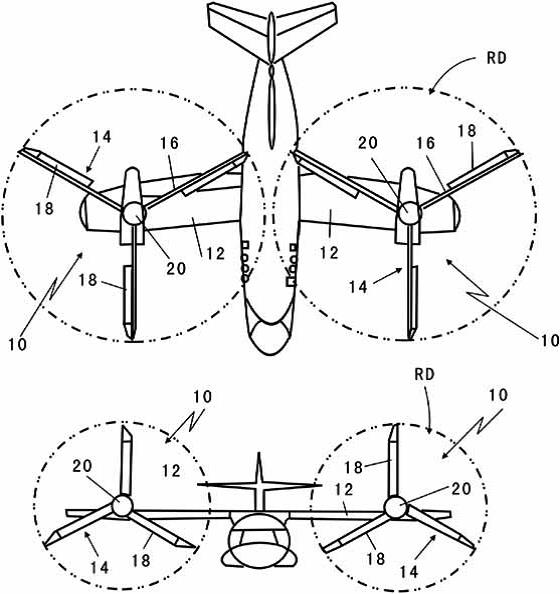
\includegraphics[height = 6cm]{Images/Litreature/TiltRotor}     
\caption{Hager's design for a telescopic tilt rotor system (Taken from \cite{Heli})}
\label{IM_EG}
\end{figure}




\begin{enumerate}
\item Flight time and efficiency
\item Geometry and size
\item Drone Manoeuvrability
\item Control algorithms
\item Mechanical complexity
\end{enumerate}

\begin{equation}
\label{EQ_EG}
DL (\frac{N}{m^{2}})= \frac{T}{A} = \frac{1}{2} \rho v_\infty^2
\end{equation}
